\documentclass{article}
\usepackage[utf8]{inputenc}
\usepackage{amsmath}
\usepackage{amssymb}
\usepackage{booktabs}
\usepackage{cancel}
\usepackage{enumitem}
\usepackage{graphicx}
\usepackage{mathtools}
\usepackage{mdframed}
\usepackage{multirow}
\usepackage{pgfgantt}
\usepackage{pdflscape}
\usepackage{appendix}
\usepackage{bbm}
\usepackage{caption} 
\usepackage{subcaption} 
\usepackage[margin=1in]{geometry}
\usepackage{biblatex} 
\addbibresource{library.bib}

\title{NE8 Lecture 3: Common transport methods}
\author{Paul Cosgrove}
\date{September 2022}

\begin{document}

\maketitle

Previously we saw the transport equation,
\begin{equation}\label{eq:transport}
    \begin{split}
 \mathbf{\Omega}\cdot\nabla\psi + \Sigma_\mathrm{tr}\psi
    =\frac{1}{4\pi}\frac{\bar{\nu}\Sigma_\mathrm{f}}{ k_\mathrm{eff}}\phi + \frac{1}{4\pi}\Sigma_\mathrm{s}\phi\;\mathrm{,}
    \end{split}
\end{equation}
and briefly discussed the P$_n$ method -- one means of solving the transport equation numerically. We briefly stated that the method is very often impractical, but we want to solve the transport equation nevertheless. This lecture will introduce some of the more common methods and discuss under which circumstances they tend to be used. In particular, the two methods introduced here are both commonly used in \textbf{lattice physics}, i.e., calculating the neutronic behaviour of fuel pins and assemblies. You will use both of them in your coursework in a few weeks time.

\section{The integral transport equation}

One simple but widely used set of methods starts from what is known as the integral transport equation -- this is as opposed to the integro-differential transport equation with which we have dealt with so far. \textbf{If we can have a purely integral transport equation, can we also have a purely differential transport equation?}

To obtain the integral equation, we first write Eq.~\eqref{eq:transport} in \textbf{characteristic form}. This means simplifying the streaming term, $\mathbf{\Omega}\cdot\nabla\psi$, by considering how this term looks from the neutrons' frame of reference. Let's say our neutrons are travelling in a particular direction, $\mathbf{\Omega}$, and arrive at position $\mathbf{r}$ starting from another position, $\mathbf{r}'$. This is visualised in Fig.~\ref{fig:integral}. We can relate all of these quantities with the distance the neutron has travelled, $s$:
\begin{equation}
    \mathbf{r}'=\mathbf{r} - s\mathbf{\Omega}\;\mathrm{,}
\end{equation}
with $s = |\mathbf{r}-\mathbf{r}'|$. This equation essentially says if our neutron travelled backwards from its final position, $\mathbf{r}$, it would reach $\mathbf{r}'$.

\begin{figure}[h]
    \centering
    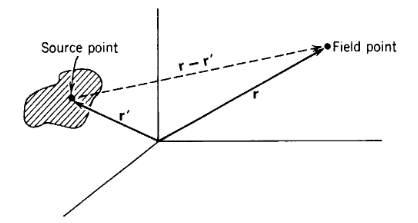
\includegraphics[width=0.6\linewidth]{integral_coordinates.png}
    \caption{Visualisation of the characteristic co-ordinate system \cite{Duderstadt}.}
    \label{fig:integral}
\end{figure}
%Alternatively, we can flip this round and talk about how far \textbf{back} neutrons must go to reach $\mathbf{r}'$ from $\mathbf{r}$:
%\begin{equation}
%    \mathbf{r} = \mathbf{r}'-s\mathbf{\Omega}\;\mathrm{.}
%\end{equation}
%We'll use both of these parameterisations in this lecture for convenience. For now, we'll focus on the second one, so 
If we write the transport equation in terms of $\mathbf{r}'$, we can write our angular flux as $\psi(\mathbf{r}',\mathbf{\Omega})=\psi(\mathbf{r}-s\mathbf{\Omega},\mathbf{\Omega})$. Applying the leakage operator to the flux gives:
\begin{equation}
    \mathbf{\Omega}\cdot\nabla \psi = -\frac{\mathrm{d}}{\mathrm{d}s}\psi\;\mathrm{,}
\end{equation}
which comes directly from the chain rule:
\begin{equation}
    \mathbf{\Omega}\cdot\nabla =\Omega_x\frac{\partial}{\partial x'} + \Omega_y\frac{\partial}{\partial y'} + \Omega_z\frac{\partial}{\partial z'} = -\frac{\mathrm{d}x'}{\mathrm{d}s}\frac{\partial}{\partial x'} - \frac{\mathrm{d}y'}{\mathrm{d}s}\frac{\partial}{\partial y'} - \frac{\mathrm{d}z'}{\mathrm{d}s}\frac{\partial}{\partial z'} = -\frac{\mathrm{d}}{\mathrm{d}s}\;\mathrm{.}
\end{equation}
As a result, the transport equation becomes much simpler:
\begin{equation}\label{eq:back_characteristic}
    -\frac{\mathrm{d}}{\mathrm{d}s}\psi(\mathbf{r}-s\mathbf{\Omega},\mathbf{\Omega}) + \Sigma_\mathrm{tr}(\mathbf{r}-s\mathbf{\Omega})\psi(\mathbf{r}-s\mathbf{\Omega},\mathbf{\Omega}) = Q(\mathbf{r}-s\mathbf{\Omega},\mathbf{\Omega})\;\mathrm{,}
\end{equation}
where we have combined the right-hand side into a single source term for compactness. This is the \textbf{characteristic form of the transport equation}. It is exact along a `characteristic' of the transport equation, that is, along the straight lines which neutrons fly. There is a characteristic equation describing every combination of $\mathbf{r}$ and $\mathbf{\Omega}$ (and energy too).

Eq.~\eqref{eq:back_characteristic} can be solved with an integrating factor solution, where the integrating factor is:
\begin{equation}
    \exp\left(-\int^s_0 \mathrm{d}s' \;\Sigma_\mathrm{tr}(\mathbf{r}-s'\mathbf{\Omega})\right)\;\mathrm{.}
\end{equation}
This gives:
\begin{equation}
    -\frac{\mathrm{d}}{\mathrm{d}s}\left[\psi(\mathbf{r}-s\mathbf{\Omega},\mathbf{\Omega})\mathrm{e}^{-\int^s_0 \mathrm{d}s' \;\Sigma_\mathrm{tr}(\mathbf{r}-s'\mathbf{\Omega})}\right]=Q(\mathbf{r}-s\mathbf{\Omega},\mathbf{\Omega})\mathrm{e}^{-\int^s_0 \mathrm{d}s' \;\Sigma_\mathrm{tr}(\mathbf{r}-s'\mathbf{\Omega})}\;\mathrm{,}
\end{equation}
which we can integrate from $s = 0$ to $s = \infty$. We neglect boundary conditions here to keep things simple, and assume that the contribution from the angular flux infinitely far away is 0. This gives:
\begin{equation}
    \psi(\mathbf{r},\mathbf{\Omega}) = \int^\infty_0\mathrm{d}s\;Q(\mathbf{r}-s\mathbf{\Omega},\mathbf{\Omega})\mathrm{e}^{-\int^s_0 \mathrm{d}s' \;\Sigma_\mathrm{tr}(\mathbf{r}-s'\mathbf{\Omega})}\;\mathrm{.}
\end{equation}
This equation tells us what the angular flux is at $\mathbf{r}$ as a result of all points upstream, $\mathbf{r}'$. 

If we assume isotropic sources (so we have $Q$ as the source pointing towards us, with $q$ as the total isotropic source -- the fraction of the isotropic source pointing towards us is then $q/4\pi$) then we can obtain an equation for the scalar flux at any point as a result of neutrons produced at all other points. We do this simply by integrating over angle:
\begin{equation}
    \phi(\mathbf{r}) = \frac{1}{4\pi}\int_{4\pi}\mathrm{d}\Omega \int^{\infty}_0\mathrm{d}s\; q(\mathbf{r}-s\mathbf{\Omega})\mathrm{e}^{-\int^s_0\mathrm{d}s'\Sigma_\mathrm{tr}(\mathbf{r}-s'\mathbf{\Omega})}\;\mathrm{.}
\end{equation}
We can simplify this integration into a standard volume integral by multiplying and dividing inside the integral by $s^2$. This allows us to make the conversion:
\begin{equation}
    \int_{4\pi}\int^\infty_0 \mathrm{d}\Omega \mathrm{d}s \;s^2 = \int_\infty \mathrm{d}V \;\mathrm{,}
\end{equation}
as the left-hand side is a volume integration over all space in polar co-ordinates. Finally, (and noting that $s = |\mathbf{r} - \mathbf{r}'|$) this gives:
\begin{equation}\label{eq:integral}
    \phi(\mathbf{r}) = \int_{\infty}\mathrm{d}V'\; q(\mathbf{r}')\frac{\mathrm{e}^{-\tau_{\mathbf{r},\mathbf{r}'}}}{4\pi |\mathbf{r}-\mathbf{r}'|^2}\;\mathrm{,}
\end{equation}
where $\tau_{\mathbf{r},\mathbf{r}'}$ is the `optical distance' between the two points -- shorthand for the integral that was previously in the exponent.

This is a remarkably simple equation that can be used to calculate the neutron flux in a reactor. It can be interpreted as stating that the neutron flux at one point in space is the result of the neutrons produced at all other points in space, accounting for some proportion of those neutrons colliding and being absorbed or scattered along the way. Of course, the neutron source at every point is due to the flux at all those points, so there remains a non-linearity to resolve: this is dealt with in much the same way as with power iteration, but we'll discuss that more later.

As well as being used to derive numerical methods for estimating transport solutions, the integral transport equation also has value in providing part of the rigorous basis for Monte Carlo calculations \cite{Lux}. 

\subsection{The integral transport equation in history: the Frisch-Peierls memorandum}

In 1938, after the discovery of fission, it was not immediately appreciated that this could be used to construct a compact nuclear weapon -- in fact it was nearly agreed upon that it couldn't be practically done.

In 1939 and 1940, at the University of Birmingham, newly emigrated Otto Frisch and Rudolph Peierls were forbidden from working on anything that was considered relevant to the war effort. Instead they continued tinkering with the maths and physics of nuclear fission (which Frisch had previously helped explain and even named!).

Frisch was working on thermal diffusion for the enrichment of uranium, while Peierls was trying to derive theoretical results on what mass of uranium would be required to make a nuclear weapon -- if one could be made, it was an open question whether it would ever be practical.

Peierls published a paper in the 1939 Mathematical Proceedings of the Cambridge Philosophical Society:``Critical conditions in neutron multiplication" (which you can find on Moodle!). Assuming neutrons are monoenergetic (fast), he derives the following expression for the number of neutrons at one point in space (and time) compared to another:
\begin{equation}
    n(x,y,z,t) = \frac{\beta}{4\pi}\int n\left(x',y',z',t-\frac{R}{c}\right)\frac{\mathrm{e}^{-\alpha R}}{R^2}\mathrm{d}x'\mathrm{d}y'\mathrm{d}z'\;\mathrm{,}
\end{equation}
where $n$ is the number of neutrons at a point in space and time, $\beta = \Sigma_\mathrm{s}+\nu\Sigma_\mathrm{f}$, $R = s$, $c$ is the neutron speed, and $\alpha=\Sigma_\mathrm{t}$.

With this familiar looking (albeit time-dependent) equation he was able to examine the possibility of constructing a nuclear weapon based on the fast fission of natural uranium. On inserting the understood properties of uranium at the time he found that a bomb would require many tons of uranium to reach criticality -- making it completely impractical to design, deliver, and detonate.

It was Frisch who realised that $^{235}$U had a much more favourable set of cross sections than $^{238}$U. On inserting the best estimates of its cross sections at the time into Peierls' equation, he found that only 1 kg of $^{235}$U would be required to reach criticality! The actual (uncompressed) critical mass is 52 kg, but this calculation was enough to show that a nuclear bomb is possible, prompting them to write the Frisch-Peierls memorandum, starting the British weapons effort and ultimately leading to the Manhattan project. So the equations in this course do have some practical use!

\begin{figure}[h]
    \centering
    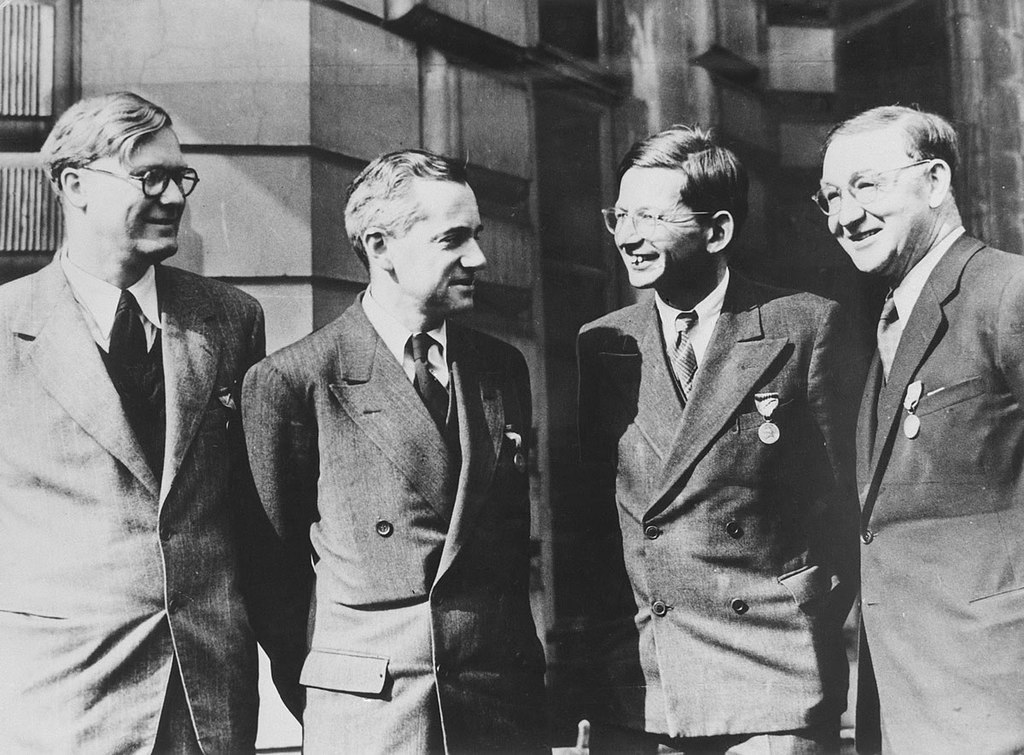
\includegraphics[width=0.6\linewidth]{physicists.jpg}
    \caption{From left to right: William Penney, Otto Frisch, Rudolph Peierls, and John Cockroft.}
    \label{fig:frisch}
\end{figure}

\subsection{The Collision Probability Method (CPM)}
We return now to how we numerically solve the integral transport equation, 
\begin{equation*}
    \phi(\mathbf{r}) = \int_{\infty}\mathrm{d}V'\; q(\mathbf{r}')\frac{\mathrm{e}^{-\tau_{\mathbf{r},\mathbf{r}'}}}{4\pi |\mathbf{r}-\mathbf{r}'|^2}\;\mathrm{.}
\end{equation*}
We begin this by discretising our space, e.g., by  making a mesh where we assume certain properties of each mesh region are uniform, as we do in all deterministic methods. Each mesh region, $i$, has an associated volume, $V_i$. This lets us define the average flux in a region as:
\begin{equation}
    \phi_i = \frac{1}{V_i}\int_{V_i}\mathrm{d}V \phi(\mathrm{r})\;\mathrm{,}
\end{equation}
and likewise the average source as:
\begin{equation}
    q_i = \frac{1}{V_i}\int_{V_i}\mathrm{d}V q(\mathrm{r})\;\mathrm{.}
\end{equation}
The impact on accuracy of treating these quantities as uniform across a mesh should decrease as the mesh becomes more finely divided.

These assumptions turn the integration over all space in Eq.~\eqref{eq:integral} into a sum of integrations over all regions. If we then integrate both sides over $V_i$ and multiply by $\Sigma_{\mathrm{tr},i}$ we obtain:
\begin{equation}
    V_i \Sigma_{\mathrm{tr},i} \phi_i = \sum_j V_j q_j P_{i,j}\;\mathrm{,} 
\end{equation}
where $P_{i,j}$ is the probability for a neutron born in region $j$ to collide in region $i$. This is actually very complicated looking and is defined as:
\begin{equation}
    P_{i,j} = \frac{\Sigma_{\mathrm{tr},i}}{V_i}\int_{V_i}\mathrm{d}V\int_{V_j}\mathrm{d}V' \frac{\mathrm{e}^{-\tau_{\mathbf{r},\mathbf{r}'}}}{4\pi|\mathbf{r}-\mathbf{r'}|^2}\;\mathrm{.}
\end{equation}
For convenience we also defined a `reduced' collision probability which is simply $p_{i,j}=P_{i,j}V_{j}/\Sigma_\mathrm{tr,i}$, giving a less ugly equation:
\begin{equation}
    \phi_i = \sum_j q_j p_{i,j}
\end{equation}
%\begin{equation}
%    \phi_i  = \sum_{j} q_j \frac{1}{V_i}\int_{V_i}\mathrm{d}V\int_{V_j}\mathrm{d}V'\frac{\mathrm{e}^{-\tau_{\mathbf{r},\mathbf{r}'}}}{4\pi|\mathbf{r}-\mathbf{r'}|}\;\mathrm{.}
%\end{equation}
While we had to go through some algebra to get here, this equation has a useful interpretation: the flux in region $i$ results from summing neutron sources in all the regions multiplied by \textbf{the probability that those neutrons make it to anywhere in region} $i$. This is exactly what the double integral term represents and, even better, it can be calculated either analytically or numerically! Essentially, estimating the fluxes in all regions (a vector $\Phi$) turns into multiplying a matrix of collision probabilities, $\mathbf{P}$, by a source vector, $\mathcal{Q}$:
\begin{equation}
    \Phi = \mathbf{P}\mathcal{Q}\;\mathrm{.}
\end{equation}
Thus we have the collision probabilities method.




\subsection{Practicalities of CPM}

As we will see in two weeks, we often want to perform many rapid calculations on 2D fuel pin problems or small portions of 2D fuel assemblies so we can get a good estimate of the neutron spectrum. This is exactly the domain where CPM excels.

\textbf{Pros:} 
\begin{itemize}
    \item If the collision probabilities from one region to another are analytically known or easy to compute, there is no angular discretisation or associated error to concern ourselves with -- this is the case in some geometries of interest (such as slabs). Symmetries in the problem (e.g., for cylindrical geometries) can also accelerate this procedure.
    \item If there are few regions in the problem, the calculation can be performed quite quickly -- since CP does not feature angles, there are fewer equations to solve.
    \item The method can also be performed, in principle, with an exact representation of the geometry, as opposed to on a mesh made of triangles or rectangles.
\end{itemize} 

\textbf{Cons:} 
\begin{itemize}
    \item The biggest problem of CPM is that it results in a \textbf{dense} matrix, connecting every region to every other region, for each energy group -- this is because its integral nature makes it non-local (as opposed to discretisations of differential operators which are local, as you will have seen in the diffusion coursework). The computational expense of dense matrix multiplication grows as $\mathcal{O}(n^2)$ and quickly becomes impractical, even for some assembly calculations. The memory footprint of the matrix may also become substantial.
    \item While collision probabilities can be estimated analytically for some geometries, these geometries are often not exactly those we are interested in. Therefore we either have to make approximations which add error (like pretending our square pin cell looks roughly like a concentric cylinder) or, for general geometries, compute collision probabilities separately. In the latter case, this adds computational expense to the method, as well as discretisation error -- the usual method for estimating collision probabilities is by ray tracing across the geometry, and if the ray laydown is not sufficiently fine then these estimates will be biased.
    \item There is no straightforward means of handling anisotropic scattering with CPM.
\end{itemize}

For these reasons, larger scale neutronics problems tend to prefer other methods.

\section{The Method of Characteristics (MoC)}

While the CPM is used for small-scale (fuel pin) reactor problems, an alternative is required for assembly-scale calculations. This is most often the Method of Characteristics (MoC). It shares many similarities with CPM but, importantly, \textbf{MoC avoids constructing a matrix}.

We derive it using a similar approach to CPM. We do this by flipping around our parameterisation of neutron position above: consider a neutron starting at $\mathbf{r}'$ in direction $\mathbf{\Omega}$. After a distance $s$ it reaches some point $\mathbf{r}$. If we stick this into the transport equation as before, we get the same simplification as before (just without the minus sign):
\begin{equation}
    \frac{\mathrm{d}}{\mathrm{d}s}\psi(s) + \Sigma_\mathrm{tr}\psi(s) = Q(s)\;\mathrm{.}
\end{equation}
This is just another way of obtaining the characteristic form of the transport equation that happens to be more convenient for our purposes.

Instead of going all the way to the integral transport equation, we make our approximations now:
\begin{itemize}
    \item Neutron sources are isotropic (this could be relaxed).
    \item The problem is discretised into regions where the neutron source and cross sections are spatially uniform (known as the flat source approximation and can also be relaxed).
    \item We only consider a discrete set of neutron directions (known as the discrete ordinates approximation).
\end{itemize}

The discrete ordinates approximation is extremely common in neutron transport. This is essentially the discretisation of the angular variables such that we only consider the transport equation along a specific set of discrete angles, $\mathbf{\Omega}_m$, each with a chosen `weight', $w_m$, such that we can replace angular integrals with summations:
\begin{equation}
	\int_{4\pi}\mathrm{d}\Omega \approx \sum^M_{m = 1} w_m = 4\pi\;\mathrm{,} 
\end{equation}
letting us approximate the scalar flux as:
\begin{equation}
	\phi \approx \sum^M_{m=1} \psi(\mathbf{\Omega}_m)w_m\;\mathrm{.}
\end{equation}
We will discuss this further in the next lecture.

The idea behind MoC is that we can solve the transport equation along each of these characteristic equations separately and then stitch the answers together to solve the full transport equation. Each of these equations essentially describes the neutron flux of a ray pointing in a particular direction from a particular starting location. To solve it, we lay tracks down all across our problem domain and solve the transport equation along one segment of the track at a time. An example of this is shown in Fig.~\ref{fig:track}. This shows solving several tracks starting at different positions but pointing in the same direction. In general, we solve equations starting at many different positions and with many different directions.

\begin{figure}[h]
    \centering
    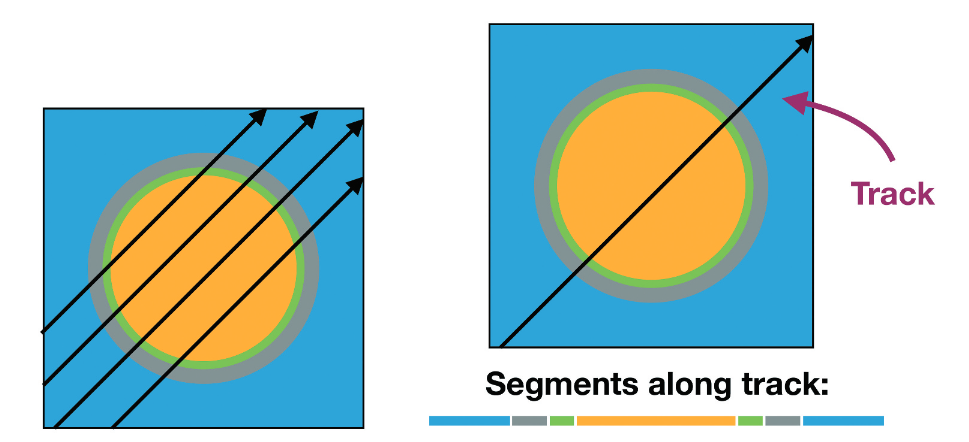
\includegraphics[width=0.9\linewidth]{tracks_segments.png}
    \caption{A few characteristic tracks laid across a pin cell problem and the division of one track into several segments over which the solution occurs \cite{Gaston2021}.}
    \label{fig:track}
\end{figure}

The analysis proceeds by considering the characteristic equation across a single flat source region. This equation now represents what happens to the angular flux as a characteristic `ray' traverses a region with uniform properties where $\mathbf{r}'$ now represents the point where the ray enters the region. Once again, we can solve this with an integrating factor, $\mathrm{e}^{\Sigma_\mathrm{tr}s}$. Integrating, setting the boundary condition at $s=0$ as $\psi_0$ (the flux the ray has as it enters the mesh) and sparing you the algebra gives:
\begin{equation}
    \psi(s) = \psi_0\mathrm{e}^{-\Sigma_\mathrm{tr}s} + \frac{Q}{\Sigma_\mathrm{tr}}\left(1-\mathrm{e}^{-\Sigma_\mathrm{tr}s}\right)\;\mathrm{.}
\end{equation}
This equation is saying that the flux along the ray after a distance $s$ is a combination of the attenuated flux that entered the mesh and the neutrons that have been picked up from sources along the way. We can also rearrange it slightly to have a simple expression for the change in angular flux across the mesh region (assuming $s$ is the whole distance the ray travels across the region):
\begin{equation}\label{eq:delta}
	\Delta\psi = \psi_0 - \psi(s) = \left(\psi_0 - \frac{Q}{\Sigma_\mathrm{tr}}\right)\left(1-\mathrm{e}^{-\Sigma_\mathrm{tr}s}\right)\;\mathrm{.} 
\end{equation} 

This equation is useful because we can use it to estimate the average angular flux in every mesh region, across many different directions and that can be used to estimate the scalar flux. The scalar flux in a chosen volume, $i$, is given by:
\begin{equation}
	\phi_i = \frac{\int_{V_i}\mathrm{d}V\int_{4\pi}\mathrm{d}\Omega\;\psi}{V_i}\approx \frac{1}{V_i}\sum_c w_c t_c L_c \bar{\psi}_c\;\mathrm{.}
\end{equation}
Here $c$ is the index of a given characteristic track across the region $i$, $w_c$ is the weight of the track in the angular quadrature, $L_c$ is the distance it covers across that region, $t_c$ is the `thickness' the track or the distance between rays going the same direction, and $\bar{\psi}_c$ is the average angular flux across the track. Note that if we sum up enough characteristics going along a region we should be able to estimate the volume of the region as $V_i \approx \sum_c w_c L_c t_c$. The concept of a track having a thickness and integrating up to the volume of the region is shown in Fig.~\ref{fig:spacing}. There is often a mismatch between the true volume and the integrated volume, but this is straightforward to correct.

\begin{figure}[h]
    \centering
    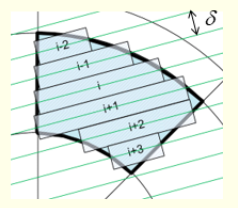
\includegraphics[width=0.3\linewidth]{ray_spacing.png}
    \caption{An illustration of the implied width of rays and how they integrate to approximate a region's volume (taken from Han-Gyu Joo's lectures on MoC).}
    \label{fig:spacing}
\end{figure}

We can calculate the average angular flux along a track multiplied by the track length as:
\begin{equation}
    L_c\bar{\psi} = \int^{L_c}_0 \mathrm{d}s\left(\psi_0\mathrm{e}^{-\Sigma_\mathrm{tr}s}+\frac{Q}{\Sigma_\mathrm{tr}}\left(1-\mathrm{e}^{-\Sigma_\mathrm{tr}s}\right)\right) = \frac{Q}{\Sigma_\mathrm{tr}} + \frac{1}{\Sigma_\mathrm{tr}}\left(\psi_0-\frac{Q}{\Sigma_\mathrm{tr}}\right)\left(1-\mathrm{e}^{-\Sigma_{tr}L_c}\right) = \frac{Q}{\Sigma_\mathrm{tr}} + \frac{\Delta\psi_c}{\Sigma_\mathrm{tr}}\;\mathrm{.}
\end{equation}
As a result, the scalar flux can be calculated as:
\begin{equation}\label{eq:MOC_flux}
	\phi_i = \frac{4\pi Q_i} {\Sigma_{\mathrm{tr},i}} + \frac{1}{V_i\Sigma_{\mathrm{tr},i}}\sum_c w_c t_c \Delta\psi_c\;\mathrm{.}
\end{equation}

Putting all this together, these equations imply a very neat way of doing a transport calculation:
\begin{enumerate}
	\item Trace rays across the reactor geometry of interest, starting at many different points on the boundary and at many different angles, remembering the distances across each cell they cross
	\item Set all $\phi_i = 0$
	\item Given an initial boundary angular flux, move along the ray
	\item Knowing the length of the track in the current cell, calculate $\Delta\psi$ according to Eq.~\eqref{eq:delta}. \textbf{This is the most computationally expensive bit because you must repeatedly evaluate an exponential!}
	\item Use this value of $\Delta\psi$ to increment $\phi_i$
	\item Continue until the end of the ray -- and then do the same but in the opposite direction!
	\item Obtain a final estimate for $\phi_i$ according to Eq.~\eqref{eq:MOC_flux}.
\end{enumerate}
This process is known as a \textbf{transport sweep} because we are sweeping across the geometry and, importantly, are \textbf{never building a matrix or storing the angular fluxes} (other than the angular fluxes at the boundaries). This greatly reduces the memory footprint and runtime of MoC on medium-to-large general geometry problems compared to methods which do not sweep. Transport sweeps are fundamental to modern deterministic methods in neutronics.

This transport sweep might have to be iterated if the boundary flux isn't known exactly, e.g., if the boundary is reflective. Then one would sweep back and forward until estimated boundary fluxes have converged between iterations. These iterations are then done inside the usual neutronics power iteration.

MoC was historically performed for lattice calculations, i.e., 2D assembly problems. MoC was favoured in this circumstance because it (and CPM if it uses ray tracing) can handle exact geometries: one can avoid linearising curved edges in reactor problems. 

Neutrons always travel in 3D, but if we analyse 2D problems we can be clever and save computation by only tracing rays in the 2D plane. This means that as we traverse the ray we perform the same calculations for different \textbf{polar} angles as well, each with a \textbf{different weight and different length}. An example of how the full MoC transport sweep tends to look is shown in Fig.~\ref{fig:sweep}.

\begin{figure}[h]
    \centering
    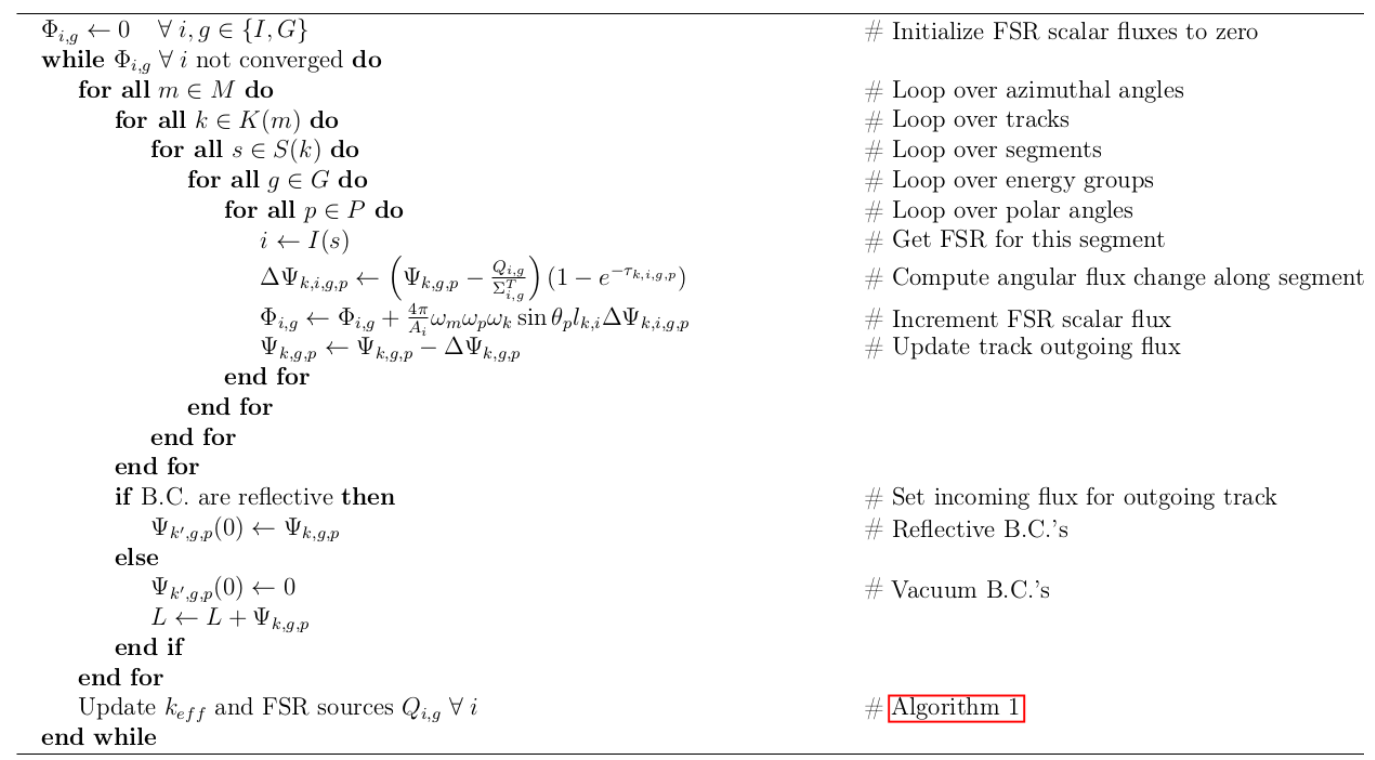
\includegraphics[width=0.9\linewidth]{sweep.png}
    \caption{The MoC transport sweep as described by OpenMOC (note extra weight variables and sine scaling due to including polar angles) \cite{openmoc}.}
    \label{fig:sweep}
\end{figure}

\begin{figure}[h]
    \centering
    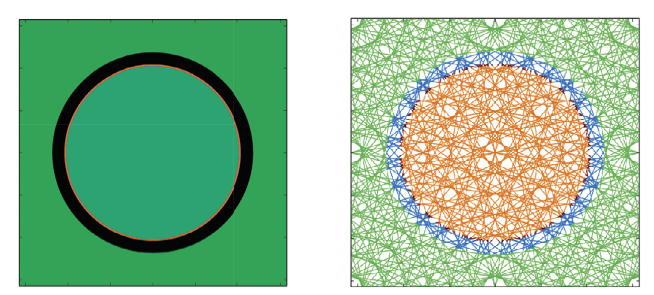
\includegraphics[width=0.9\linewidth]{cyclic.png}
    \caption{A cyclic track laydown in a pin cell problem. Cyclic tracking is a convenient way to allow boundary conditions to be met (e.g., reflective boundaries) \cite{Tramm2017}.}
    \label{fig:laydown}
\end{figure}

Both the accuracy and computational intensity of MoC are controlled by how tightly one lays down the rays across the geometry, how many azimuthal (in-the-plane) and polar (out-of-the-plane) angles these rays cover (to mitigate the discrete ordinates approximation), and how finely discretised the geometry is (to mitigate the flat source approximation). An example track laydown is shown in Fig.~\ref{fig:laydown}: this is \textbf{far} too coarse to give an accurate answer. In reasonable fidelity MoC calculations, a visualisation of the laydown tends to be completely black with rays! An example (reasonable) geometry discretisation is shown in Fig.~\ref{fig:disc}. for a single assembly problem surrounded by a water gap.

\begin{figure*}[h!]
     \centering
    \begin{subfigure}[t]{0.45\textwidth}%
    \captionsetup{justification=centering}
         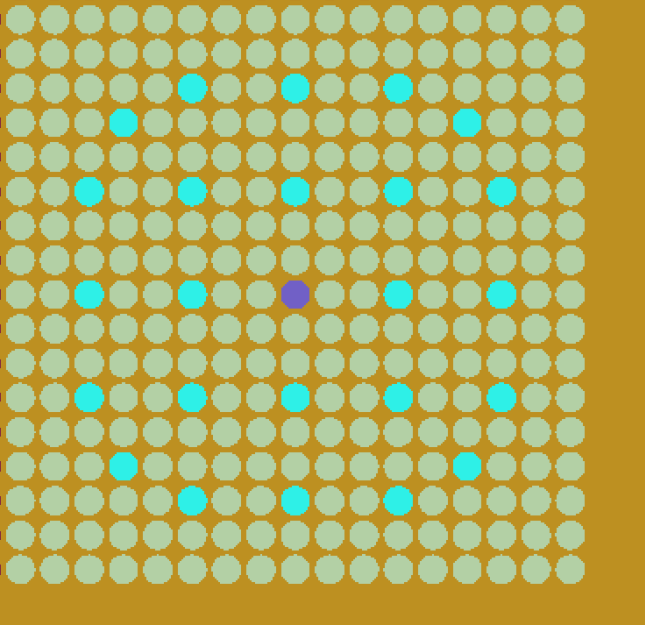
\includegraphics[scale=0.65]{assembly.png}%
         \caption{A single PWR assembly surrounded by water}
         \label{fig:C5G7}
    \end{subfigure}
    \begin{subfigure}[t]{0.45\textwidth}
    \captionsetup{justification=centering}
         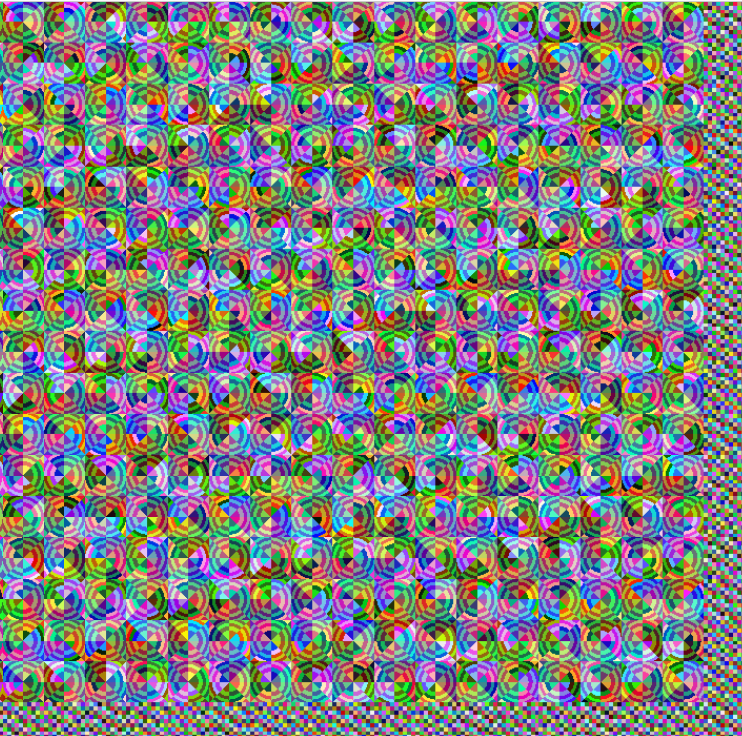
\includegraphics[scale=0.555]{assembly_disc.png} 
	       \caption{The discretisation of the assembly in standard calculations} 
	       \label{fig:MGMC_cells}
    \end{subfigure}
  
    \caption{MoC geometry and its discretisation}
    \label{fig:disc}
\end{figure*}

The MoC literature has evolved quite rapidly in the last two decades, driven, in part, by changes in computing hardware and increased parallelism. The independent characteristic tracks are quite well suited for this. One thing to be aware of is that older literature often states that the required ray tracing is a bottleneck to the method -- this is essentially no longer true. While, ideally, one would not ray trace the same tracks every iteration, a ray trace is not an expensive operation and ray tracing `on-the-fly' may have more advantages in reducing memory footprint and avoiding slow memory accesses than the disadvantage of costing some additional FLOPs (floating point operations).

There is much more that could be said about MoC, such as how it has been extended to handle whole core reactor calculations, but that is well beyond the scope of this course. Next lecture we will cover the $S_n$ method (which is also sweep-based) and talk a little bit more about how transport methods differ from diffusion. 

\printbibliography

\end{document}
